\section{Work Breakdown Structure}

\begin{figure}[H]
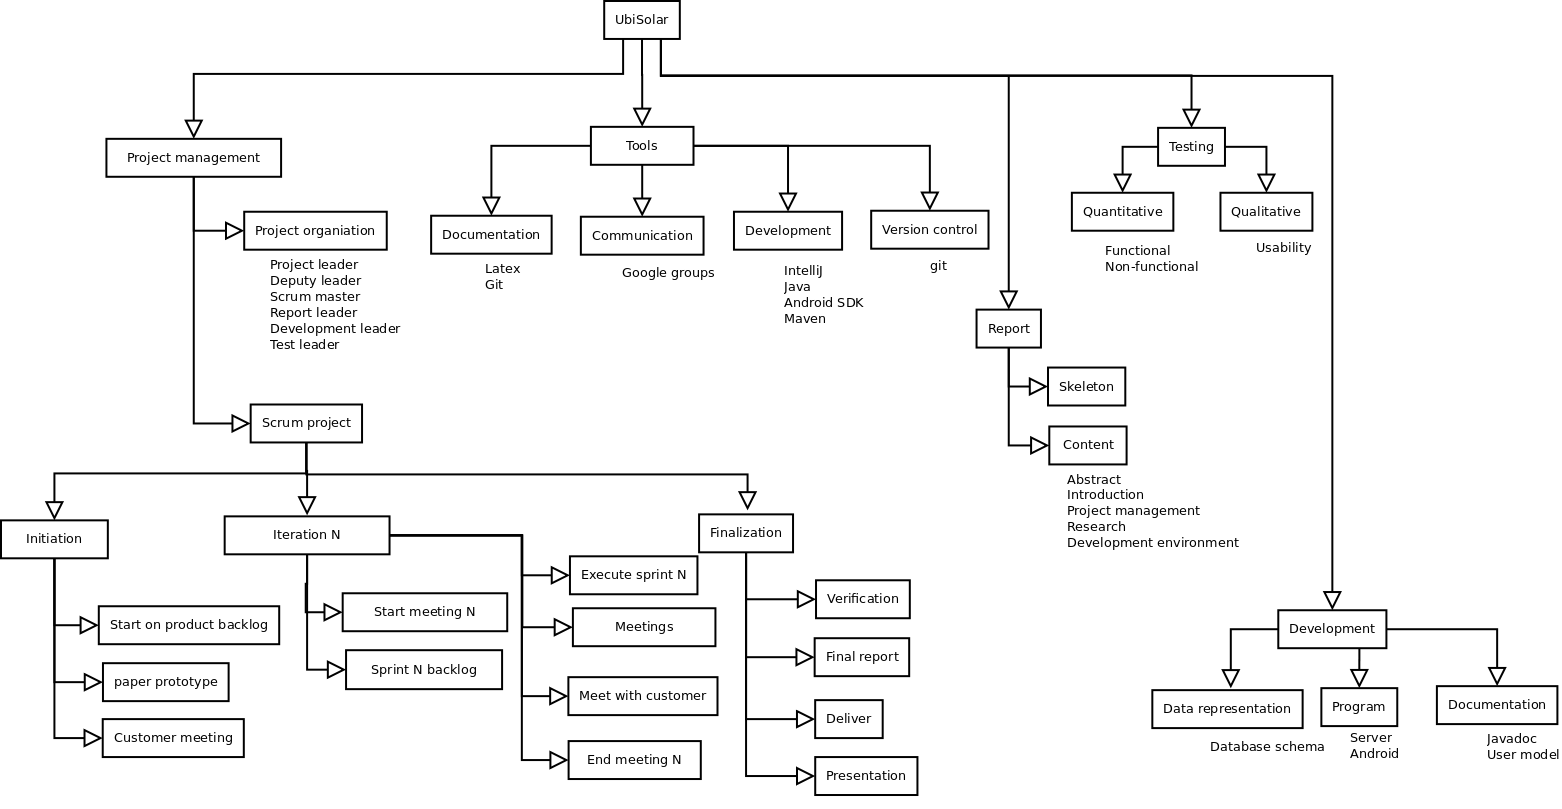
\includegraphics[width=\textwidth]{ch/projectPlan/fig/WBS.png}
\caption{The work breakdown structure. Each WBS packet is a product from the project work.}
\label{fig:wbs}
\end{figure}

The work breakdown structure \ref{fig:wbs} is broken down into five parts. Each part is a package that represents a part of the work that needs to be done in the project.
The reason for using WBS is so that the team can analyze of much time that is actually spent on the different parts of the project compared to how it was planned.
The effect of doing this is that one can easily see if some part of the project gets forgotten or gets too much time.

\begin{table}[H]
\centering
\rowcolors{1}{darkgray}{lightgray}
\begin{tabular}{l c r}
    \textbf{WB \#} & \textbf{Name} & \textbf{Hours} \\\hline
    1 & Project management & .5/10 = 87\\\hline
    2 & Tools 			   & 1.5/10 = 261\\\hline
    3 & Report 			   & 4/10 = 696\\\hline
    4 & Development 	   & 3/10 = 522\\\hline
    5 & Testing  		   & 1/10 = 174\\\hline
\end{tabular}
\end{table}

From the total amount of hours for project, the team has broken up each WBS packet in a fraction, based on how much time the team should use one the given part.

For each sprint the time can see how much time that has been spent on each packet, and if time is beeing distributed according to the planned amount of time on each packet.